\chapter{Implementación de la Solución}

En este capítulo se presentan los detalles de implementación de un sistema centralizado cuyo objetivo es aproximar el estado del tráfico en tiempo real. La solución propuesta está basada en FCD obtenido mediante dispositivos móviles. La información resultante es almacenada en una base de datos GIS y se encuentra disponible para consultas a través de una aplicación móvil y una página web desarrolladas para el efecto.

\section{Arquitectura}

En la \Cref{fig:arquitectura} se ilustra la arquitectura modular del sistema desarrollado. La plataforma cuenta con tres componentes principales:
\begin{enumerate*}[1)] \item una base de datos GIS que almacena el mapa de calles y las trayectorias de los vehículos, \item una aplicación móvil que captura los datos del trayecto recorrido por los vehículos y \item una aplicación web que procesa los datos obtenidos y genera información sobre el estado del tránsito.
\end{enumerate*}

\begin{figure}[h*]
	\centering
	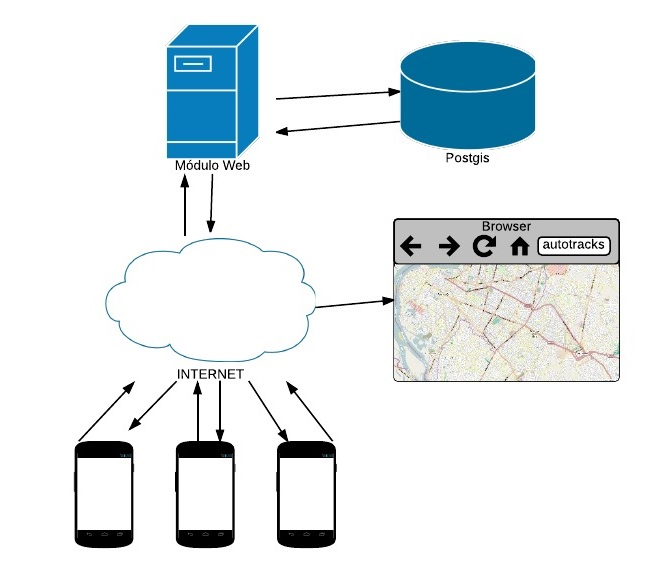
\includegraphics[width=0.7\textwidth]{capitulos/6/figuras/figura1.jpg}
	\caption{\label{fig:arquitectura} Arquitectura del Sistema}	
\end{figure}

Para el almacenamiento de la información se utiliza el motor de base de datos PostgreSQL\footnote{http://www.postgresql.org/} al que además se agregan las extensiones PostGIS\footnote{http://postgis.net/}, que añade capacidades GIS, y pgRouting\footnote{http://pgrouting.org/}, que añade funciones de ruteo geoespacial. Por otro lado, con el propósito de recolectar la información de FCD se cuenta con una aplicación móvil desarrollada para sistemas operativos Android\footnote{http://developer.android.com/index.html} 2.3 o superior, que se ejecuta en los dispositivos de los usuarios. Por último, para el procesamiento y recuperación de la información se cuenta con una aplicación web desarrollada con tecnología Java EE\footnote{http://docs.oracle.com/javaee/} que implementa servicios REST a través de los cuáles la aplicación móvil envía y obtiene datos del servidor.

\section{Almacenamiento de datos}
\label{base-de-datos}

A modo de generar información sobre el estado del tráfico de un área geográfica en particular, se debe contar con un mapa de calles y con un conjunto de trayectorias obtenidas mediante FCD durante un período de tiempo determinado. El mapa y las trayectorias deben estar almacenados en la base de datos GIS para posteriormente ser utilizados durante el procesamiento de la información.

Primeramente, para el mapa de calles se utilizan los datos geográficos disponibles en Open Street Maps\footnote{http://www.openstreetmap.org/} (OSM). Los datos descargados desde OSM están en el formato OSM XML, el cual consiste en una lista de instancias de nodos, caminos y relaciones dentro de su modelo. Antes de almacenar estos datos es necesario transformarlos a un formato soportado por PostGIS y pgRouting. pgRouting representa toda la información de las rutas como un grafo dirigido, donde los vértices corresponden a las intersecciones de las calles y las aristas corresponden a los segmentos de calles, la longitud de la calle determina su peso, que es utilizado para el cálculo del camino más corto. Para convertir e importar los datos de OSM a la base de datos se utiliza la herramienta osm2po\footnote{http://osm2po.de/} y como resultado de esta importación se crea una tabla en la que cada fila corresponde a un segmento de calle. 

Por otro lado, para almacenar la información de las trayectorias de los usuarios se definen las siguientes tablas:
\begin{enumerate}
\item \textbf{Localizaciones}: En esta tabla se guardan los datos de ubicación que son recibidos periódicamente de los usuarios de la aplicación móvil. Se almacena la fecha, la latitud, la longitud, la velocidad, la dirección, la precisión, altitud y la ruta a la que pertenece. Las localizaciones representan los puntos de una trayectoria.
\item \textbf{Rutas}: Una ruta es un conjunto de localizaciones que sirven como dato de entrada para el proceso de MM. La ruta representa a la trayectoria recorrida por el usuario durante un viaje.
\end{enumerate}

Todos los datos geométricos, tanto del mapa de calles como de las trayectorias, son almacenados utilizando un sistema de coordenadas WGS84 conforme se describe en el \cref{sistema_de_coordenadas}.

\section{Implementación de FCD}
\label{floating-car-data}

La información de FCD es obtenida por medio de una aplicación móvil desarrollada como parte del presente trabajo que ha sido denominada Autotracks\footnote{https://play.google.com/store/apps/details?id=py.com.fpuna.autotracks}. La misma se encarga de capturar, almacenar y enviar periódicamente a un servidor central las trayectorias de los usuarios, además la aplicación sólo captura las localizaciones mientras los usuarios están en un vehículo en movimiento. Para este propósito, Autotracks cuenta con tres componentes principales: 
\begin{itemize}
	\item Reconocimiento de actividad.
	\item Toma de localizaciones.
	\item Envío de datos.
\end{itemize}

\subsection{Reconocimiento de actividad}
\label{reconocimiento_actividad}

El reconocimiento de actividad consiste en determinar la acción que está realizando una persona en base a un patrón de movimientos observados para dicha persona, estas actividades pueden ser por ejemplo una caminata, un paseo en bicicleta, etc. Para realizar el reconocimiento de actividad se pueden utilizar los sensores con los que cuentan los dispositivos móviles, como el acelerómetro, el giroscopio y los dispositivos GPS integrados. En Autotracks se utiliza el reconocimiento de actividad para determinar cuando un usuario se encuentra en un vehículo en movimiento.

En \cite{liao2006location,bao2004activity,ravi2005activity} se describen técnicas que permiten detectar la actividad mediante los sensores GPS y el acelerómetro de los dispositivos móviles. En \cite{thiagarajan2010cooperative} se utilizan estas técnicas de reconocimiento de actividad para determinar si el usuario está en un vehículo en movimiento. En Autotracks, en lugar de implementar un algoritmo de reconocimiento de actividad propio, se reutiliza una implementación proveída como parte de Google Play Services\footnote{http://developer.android.com/google/play-services/index.html}, denominada Activity Recognition\footnote{http://developer.android.com/training/location/activity-recognition.html}.

Autotracks consulta periódicamente la actividad del usuario, cuando se ha detectado que el usuario se encuentra en un vehículo en movimiento se inicia el servicio de toma de localizaciones, este servicio permanece activo mientras el usuario se encuentra en movimiento. El intervalo de tiempo utilizado en la detección de actividad del usuario es de 15 segundos. Una vez que se ha detectado que el usuario ya no está en movimiento durante más de 10 minutos, el servicio de toma de localizaciones es detenido. Se utiliza la tolerancia de 10 minutos para evitar que el servicio se detenga cuando el vehículo se encuentra momentáneamente detenido en espera de algún evento, como en un semáforo en rojo, esperando por alguna persona o en un embotellamiento. Los valores utilizados en la detección de actividad fueron determinados empíricamente.

El \Cref{alg:deteccion_actividad} muestra el procedimiento ejecutado periódicamente cada vez que se obtiene un resultado del reconocimiento de actividad. Este procedimiento verifica si la toma de localizaciones está o no iniciado y se encarga de iniciarla o finalizarla de acuerdo a la actividad detectada, utilizando los procedimientos $RastreoIniciado()$, $IniciarRastreo()$ y $FinalizarRastreo()$. El resultado de la detección de movimiento es almacenado para ser utilizado en la siguiente invocación del procedimiento, utilizando los procedimientos $GuardarEstabaEnMovimiento()$ y $ObtenerEstabaEnMovimiento()$. Si se ha detectado movimiento, el tiempo en el que ocurrió la detección también es almacenado para utilizarlo en la siguiente invocación, utilizando los procedimientos $GuardarUltimaDeteccion()$ y $ObtenerUltimaDeteccion()$.
 
\begin{algorithm}
\caption{Reconocimiento de Actividad}
\label{alg:deteccion_actividad}
\begin{algorithmic}[1]
\Procedure {ActividadDetectada}{$actividad$}
	\State $enMovimiento \leftarrow EstaEnMovimiento(actividad)$
	\State $GuardarEstabaEnMovimiento(enMovimiento)$
	\If {$enMovimiento$}
		\If {$\neg RastreoIniciado()$}
			\State $IniciarRastreo()$
		\EndIf
	\Else
		\If {$RastreoIniciado()$}
			\State $FinalizarRastreo()$
		\EndIf
	\EndIf
\EndProcedure
\Statex
\Procedure {EstaEnMovimiento}{$actividad$}
	\State $tiempo \leftarrow ObtenerTiempoActual()$
	\If {$actividad = A_PIE$}
		\State \Return $FALSO$
	\EndIf
	\If {$actividad = EN_VEHICULO$}
		\State $GuardarUltimaDeteccion(tiempo)$
		\State \Return $VERDADERO$
	\EndIf
	\If {$ObtenerEstabaEnMovimiento()$}
		\State $ultimaDeteccion \leftarrow ObtenerUltimaDeteccion()$
		\State $tiempoTranscurrido \leftarrow tiempo - ultimaDeteccion$
		\State \Return {$tiempoTranscurrido <= TOLERANCIA$}
	\EndIf
	\State \Return $VERDADERO$
\EndProcedure
\end{algorithmic}
\end{algorithm}

\subsection{Toma de localizaciones}
\label{toma_localizaciones}

Para obtener la ubicación de los teléfonos móviles existen varias opciones posibles, cada una con sus ventajas y desventajas, estas son: 
\begin{itemize}
\item \textbf{Triangulación de antenas}: Utiliza las antenas de telefonía para determinar la posición. Requiere un uso mínimo de batería pero produce resultados de baja precisión, dependiendo de la técnica utilizada la precisión varía de 50 a 200 metros en áreas urbanas, y hasta más de 2 kilómetros en zonas suburbanas.
\item \textbf{WiFi}: Utiliza las posiciones conocidas de los puntos de acceso Wifi para estimar la ubicación. El uso de la batería es moderado y produce resultados con una precisión de menos de 50 metros. No es apropiado para zonas rurales donde existen una escasa cantidad de puntos de acceso Wifi.
\item \textbf{GPS}: Utiliza la red de satélites GPS para obtener la posición del dispositivo. Este mecanismo requiere un alto consumo de batería y su precisión es de menos de 10 metros en el mejor caso. La precisión disminuye considerablemente cuando se pierde la visibilidad de los satélites.
\end{itemize}
A fin de tener la mayor flexibilidad posible, Autotracks es capaz de trabajar con cualquiera de estas opciones para obtener la ubicación de los dispositivos. Para ello se reutiliza una implementación denominada Fused Location Provider\footnote{http://developer.android.com/training/location/receive-location-updates.html} que está disponible como parte Google Play Services.

En los casos en los que la localización es obtenida a través de las redes GSM o WiFi no se dispone de la información de velocidad, la cual es necesaria para el procesamiento posterior. Para paliar esta falta de información, la velocidad es estimada utilizando la localización anterior de la siguiente manera: \begin{equation} \label{eq:velocidad} v=\frac { d }{ t } \end{equation} donde $d$ es la distancia entre la localización actual y la anterior, y $t$ es el tiempo que transcurrió entre la toma de las localizaciones.

Algunas de las localizaciones capturadas pueden llegar a ser demasiado imprecisas como para ser utilizadas en el procesamiento posterior. Para evitar este tipo de localizaciones erróneas se utilizan dos técnicas de filtrado. El primer método consiste simplemente en descartar las localizaciones que reportan una precisión mayor a 200 metros. El segundo método consiste en determinar la velocidad a la que tuvo que haber viajado el vehículo para pasar de la posición anterior a la posición actual utilizando la \cref{eq:velocidad}, si dicha velocidad es mayor a un valor preestablecido, en este caso de 140 km/h, la localización es descartada. Los valores de referencia fueron determinados empíricamente en sucesivas pruebas de campo.

Otro aspecto importante a tener en cuenta es la frecuencia con la que se toman las localizaciones. En \cite{tao2012real} se sugiere que intervalos de entre 10 y 20 segundos son los recomendados en aplicaciones prácticas. En \cite{fontaine2005part} se reivindica que intervalos de muestras más largos permiten obtener información sobre mayores distancias y reduce la probabilidad de capturar velocidades no representativas. En \cite{lou2009map,giovannini2011novel} se utilizan localizaciones con intervalos de más de 3 minutos en aplicaciones \emph{off-line}. Para lograr un balance entre la frecuencia y el consumo de batería, se establece un intervalo de 60 segundos para el muestreo utilizado en Autotracks, dicho valor también fue determinado empíricamente realizando pruebas en dispositivos de diversa gama.

\subsection{Envío de datos}

La aplicación envía los datos de las localizaciones a través de Internet a un servidor central que se encarga de almacenar y procesar la información. Para disminuir el consumo de batería ocasionado por la utilización de la red de datos móviles, los teléfonos almacenan temporalmente las localizaciones capturadas y las envían periódicamente al servidor. Luego de que un grupo de localizaciones ha sido enviado es borrado de la memoria del teléfono.

El intervalo de tiempo definido para el envío de los datos es de 15 minutos. Para disminuir el consumo de batería se utiliza el mecanismo de alarmas inexactas proveído por Android\footnote{https://developer.android.com/training/scheduling/alarms.html}. Al utilizar este tipo de alarmas, el sistema operativo sincroniza las alarmas de múltiples aplicaciones y las dispara al mismo tiempo. Esto reduce el número total de veces que el sistema debe despertar el dispositivo, reduciendo así el uso de la batería.

Para enviar las localizaciones no es necesario que el usuario haya finalizado completamente su recorrido, al momento de dispararse una alarma todas las localizaciones capturadas hasta el momento son enviadas al servidor. El resto de las localizaciones del mismo recorrido son enviadas al dispararse las siguientes alarmas. De esta forma los recorridos parciales pueden ser utilizados para estimar el estado del tráfico aproximadamente en tiempo real.

\section{Implementación de MM}
\label{implementacion_mm}

Un proceso de Map Matching (MM) es ejecutado cada vez que las trayectorias de los vehículos son enviadas desde los teléfonos móviles al servidor central para determinar el camino real recorrido por cada vehículo. Para realizar este proceso se utiliza el algoritmo propuesto por \cite{lou2009map}, conocido como ST-Matching, con las mejoras propuestas por \cite{budigm2012algorithm} y \cite{sakic2012map}. 

ST-Matching es un algoritmo topológico específicamente diseñado para funcionar de forma \emph{off-line} y con intervalos de tiempo relativamente largos entre las puntos. Su implementación es sencilla comparada con otras técnicas avanzadas como \cite{quddus2006high, newson2009hidden} y no requiere de procesamientos y cálculos matemáticos complejos. Estas características se adecuan a los requerimientos impuestos por la arquitectura de la solución propuesta. 

El algoritmo ST-Matching consta de tres partes principales: \begin{enumerate*}[a)]
\item la \emph{Selección de Candidatos},
\item el \emph{Análisis Espacial y Temporal} y
\item la \emph{Obtención del Resultado}.
\end{enumerate*}
La \Cref{fig:st-matching} muestra una descripción general del proceso cuyo resultado es almacenado en la base de datos para ser utilizado más adelante en el análisis de tráfico.

\begin{figure}[h]
	\centering
	\input{capitulos/6/figuras/figura61.pdf_tex}
	\caption[Descripción General de ST-Matching]{Descripción general del algoritmo ST-Matching.}
	\label{fig:st-matching} 
\end{figure}

\subsection{Marco conceptual base para MM}

Los datos de entrada del algoritmo de MM son la red de calles, que se describió en el \cref{base-de-datos}, y la trayectoria de un vehículo, obtenida mediante el uso de la aplicación móvil, como se explica en el \cref{floating-car-data}. El resultado de este procesamiento es una aproximación del camino real recorrido por el vehículo.

La red de calles es modelada como un grafo dirigido $G(V,E)$, donde $V$ es el conjunto de todos los vértices correspondientes a las intersecciones y extremos de los segmentos de calles, y $E$ es el conjunto de todas las aristas que representan segmentos de calles. Además, cada segmento $e \in E$ tiene como datos un identificador único $e.id$, el límite de velocidad $e.v$ de la calle, la longitud $e.l$ del segmento, el identificador del vértice inicial $e.ini$ y el del vértice final $e.fin$. En la \Cref{fig:segmentos_de_calle} se aprecia como una calle puede estar dividida en varios segmentos, donde cada segmento está comprendido entre dos vértices del mapa.

\begin{figure}[h*]
	\centering
	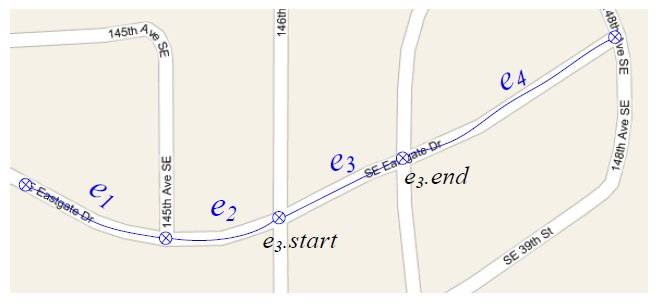
\includegraphics[width=0.8\textwidth]{capitulos/6/figuras/figura4.jpg}
	\caption{\label{fig:segmentos_de_calle} Representación de segmentos de calles}	
\end{figure}

La trayectoria $T$ de un vehículo es representada como una secuencia ordenada de puntos $p_1, p_2, \dots, p_n$ donde cada punto $p_i$ tiene además como datos su latitud $p.lat$, su longitud $p.lon$, su velocidad aproximada $p.v$, su dirección de desplazamiento $p.d$ y el tiempo $p.t$ en que fue tomada la muestra. La trayectoria está ordenada con respecto al tiempo de tal manera que $p_i.t < p_{i + 1}.t$ para $1 \le i < n$. La \Cref{fig:trayectoria} muestra un ejemplo de una trayectoria correspondiente a un vehículo de prueba.

\begin{figure}[h*]
	\centering
	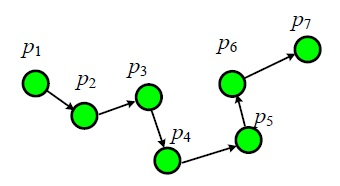
\includegraphics[width=0.5\textwidth]{capitulos/6/figuras/figura5.jpg}
	\caption{\label{fig:trayectoria} Trayectoria de un vehículo}	
\end{figure}

El camino real $R$ es definido como una secuencia de segmentos de calles $e_i$ conectados entre sí, que se inicia en un vértice $v_{ini} \in V$ y finaliza en un vértice $v_{fin} \in V$, es decir, $R = \{ e_1, e_2, \dots, e_n \}$, donde $e_1.ini = v_{ini}$, $e_n.fin = v_{fin}$ y $e_i.fin = e_{i + 1}.ini$ para $1 \le i < n$.

En base a estas definiciones, el problema de MM se puede expresar de la siguiente forma: \emph{Dada una trayectoria T y una red de calles G(V,E), encontrar el camino real R que hace coincidir a T con su reconstrucción más realista sobre G(V,E).}

\subsection{Selección de Candidatos}

La primera etapa del proceso es la selección de puntos candidatos. Un punto candidato $c$ es un punto perteneciente a un segmento de calle $e$, que puede formar parte del camino real recorrido por un vehículo, y que es obtenido a partir de un punto $p$ de una trayectoria. Dada una trayectoria $T = \{p_1, p_2, \dots, p_n\}$, el proceso de selección de candidatos consiste en encontrar para cada punto $p_i$, $1\le i\le n$, el conjunto de puntos candidatos $C_i = \{c_{i}^{1}, c_{i}^{2}, \dots, c_{i}^{m}\}$ correspondiente.

El primer paso es seleccionar todos los segmentos de calles $e \in E$ tales que la distancia entre un punto $p_i$ y un segmento $e$ sea menor a un radio $r$, de esta forma se obtiene un conjunto de segmentos $E_i = \{ e : \text{ } e \in E \text{ } \wedge \text{ } dist(p_i, e) < r \}$. Luego, para cada segmento $e_{i}^{j}$ perteneciente al conjunto $E_i = \{e_{i}^{1}, e_{i}^{2}, \dots, e_{i}^{m}\}$ resultante, se obtiene un punto candidato $c_{i}^{j}$ realizando una proyección del punto $p_i$ sobre el segmento $e_{i}^{j}$. La proyección $proy(p, e)$ de un punto $p$ sobre un segmento $e$ se define como el punto $c$ perteneciente a $e$ más cercano a $p$, es decir, $c = \text{arg } min(dist(c_i, p)) \text{ } \forall c_i \in e$. Así, se obtiene el conjunto de puntos candidatos $C_i = \{ proy(p_i, e_j) \text{ } \forall e_j \in E_i \}$. Como se puede apreciar en la \Cref{fig:puntos_candidatos} los puntos candidatos pueden ser cualquier punto del segmento, como en el caso de $c_{i}^{1}$ y $c_{i}^{2}$, o uno de sus vértices como en el caso de $c_{i}^{3}$.

\begin{figure}[h*]
	\centering
	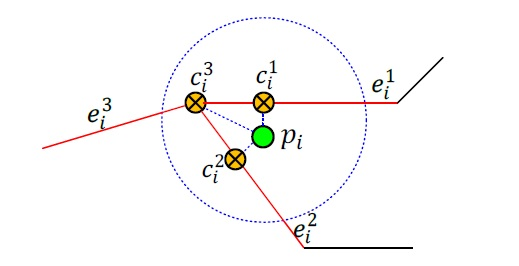
\includegraphics[width=0.5\textwidth]{capitulos/6/figuras/figura6.jpg}
	\caption{\label{fig:puntos_candidatos} Puntos candidatos para un punto de la trayectoria}	
\end{figure}

Una vez que se han obtenidos todos los conjuntos $C_i = \{c_{i}^{1}, c_{i}^{2}, \dots, c_{i}^{m}\}$ correspondientes a cada punto $p_i$ de la trayectoria $T$, el problema de MM se reduce a cómo seleccionar un punto candidato $c_i$ de cada conjunto $C_i$, a partir del cual se obtiene el segmento de calle $e_i$, de manera tal que el camino real resultante $R = \{ e_1, e_2, \dots, e_n \}$ sea lo más aproximado posible a $T = \{ p_1, p_2, \dots, p_n\}$, conforme se describe en los siguientes apartados.

\subsection{Análisis Espacial y Temporal}

La segunda etapa del proceso tiene por objetivo seleccionar el punto candidato $c_i$ de cada conjunto $C_i$ que sea el más apropiado para cada punto $p_i$ de la trayectoria. Para ello cada punto candidato y cada posible conexión entre dos puntos candidatos consecutivos, son analizados de acuerdo a dos criterios de calidad, el \emph{análisis espacial} y el \emph{análisis temporal}.

\subsubsection{Análisis Espacial}

En el análisis espacial se utiliza información geométrica y topológica de la red de calles para evaluar los puntos candidatos. La información geométrica es incorporada utilizando la \emph{probabilidad de observación} y la información topológica es expresada utilizando la \emph{probabilidad de transmisión}.

La \emph{probabilidad de observación} es la probabilidad de que un punto candidato $c_{i}^{j}$ corresponda a un punto $p_i$ de la trayectoria, calculada en base a la distancia $dist(c_{i}^{j},p_i)$ entre los puntos. Asumiendo que el error en la medición de la posición de $p_i$ sigue una distribución normal, la probabilidad de observación $N(c_{i}^{j})$ se define como
\begin{equation} \label{probabilidad_de_observacion}
N(c_{i}^{j}) = \frac {1}{\sqrt { 2 \pi \sigma }} {e}^{\frac {{(x_{i}^{j} - \mu)}^{2}}{{ 2 \sigma}^{2}}}
\end{equation}
donde $x_{i}^{j} = dist(c_{i}^{j},p_i)$ es la distancia entre $p_i$ y el punto candidato $c_{i}^{j}$. En este trabajo se utiliza una media $\pi = 50\text{m}$ y una desviación estándar $\sigma = 100\text{m}$. Estos valores fueron determinados empíricamente y son distintos a los valores utilizados en \cite{lou2009map} y \cite{budigm2012algorithm} debido a que, a diferencia de estos trabajos anteriores, no todas las muestras son obtenidas mediante el uso de GPS.

El cálculo de la probabilidad de observación tiene en cuenta únicamente la posición de los puntos $p_i$ y $c_{i}^{j}$, ignorando la topología y la posición relativa de los puntos con respecto a los demás puntos de la trayectoria. Debido a esto pueden darse casos en los que un punto candidato es seleccionado erróneamente por ser el más cercano aún cuando existen otros puntos candidatos más adecuados. Esta situación se puede presentar en las intersecciones de calles o en calles paralelas muy cercanas como se muestra en la \Cref{fig:probabilidad_transmision}.

\begin{figure}[h*]
	\centering
	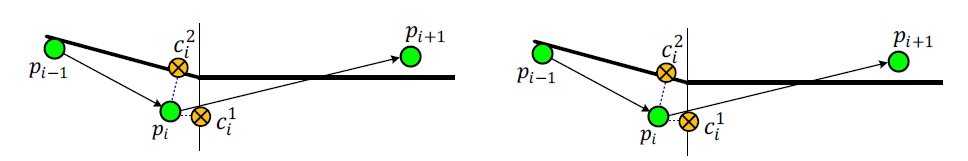
\includegraphics[width=0.9\textwidth]{capitulos/6/figuras/figura7.jpg}
	\caption{\label{fig:probabilidad_transmision} Errores en la probabilidad de observación}	
\end{figure}

Para minimizar la ocurrencia de estos problemas se introduce un segundo criterio denominado \emph{probabilidad de transmisión}, que se define como la probabilidad de que el camino más corto entre un punto candidato $c_{i-1}^{j}$ y el siguiente punto candidato $c_{i}^{k}$ es el camino correcto de $p_{i-1}$ a $p_i$. La probabilidad de transmisión se calcula de la siguiente forma: \begin{equation} \label{probabilidad_de_transmision}
V(c_{i-1}^{j}, c_{i}^{k}) = \frac { min( dist(p_{i-1}, p_i), long(c_{i-1}^{j}, c_{i}^{k})) }{ max (dist(p_{i-1}, p_i), long(c_{i-1}^{j}, c_{i}^{k})) }
\end{equation}
donde $long(c_{i-1}^{j}, c_{i}^{k})$ es la longitud del camino más corto entre $c_{i-1}^{j}$ y $c_{i}^{k}$. El cálculo del camino más corto se realiza utilizando el algoritmo de Dijkstra\footnote{http://es.wikipedia.org/wiki/Algoritmo\_de\_Dijkstra} para grafos dirigidos. La dirección de las aristas del grafo representan el sentido de circulación de la calle, de esta forma se incorpora información topológica en el análisis espacial. 

Combinando la \Cref{probabilidad_de_observacion} y la \Cref{probabilidad_de_transmision} se define la función de análisis espacial $F_s(c_{i-1}^{j},c_{i}^{k})$ como el producto de la probabilidad de observación y la probabilidad de transmisión de la siguiente forma:
\begin{equation} \label{funcion_espacial}
F_s(c_{i-1}^{j},c_{i}^{k}) = N(c_{i}^{k}) * V(c_{i-1}^{j}, c_{i}^{k}), \quad 2 \le i \le n 
\end{equation}

Como resultado del análisis espacial se asigna un valor numérico a todos los posibles caminos que van de $p_{i-1}$ a $p_i$ obtenido mediante la \Cref{funcion_espacial}.

\subsubsection{Análisis Temporal}

Existen casos en los que el análisis espacial no es suficiente para identificar un segmento de calle correctamente. En la \Cref{fig:analisis_temporal} la línea más gruesa representa a una autopista mientras que la línea más delgada representa a una calle vecinal, el límite de velocidad de la autopista es superior al de la calle vecinal cercana, utilizando sólo el análisis espacial se podría seleccionar incorrectamente una de las dos. Para evitar esto se calcula la velocidad promedio entre dos puntos consecutivos $p_{i-1}$ y $p_i$ y se compara con los límites de velocidad promedio de los segmentos de calles comprendidos entre dos puntos candidatos $c_{i-1}^{j}$ y $c_{i}^{k}$ con el fin de seleccionar el segmento cuya velocidad promedio es la más cercana a la velocidad promedio de desplazamiento del vehículo.

\begin{figure}[h*]
	\centering
	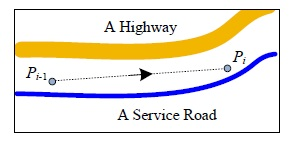
\includegraphics[width=0.6\textwidth]{capitulos/6/figuras/figura8.jpg}
	\caption{\label{fig:analisis_temporal} Error en el análisis espacial}	
\end{figure}

Dados dos puntos candidatos $c_{i-1}^{j}$ y $c_{i}^{k}$ correspondientes a dos puntos consecutivos $p_{i-1}$ y $p_i$ respectivamente, el camino más corto entre $c_{i-1}^{j}$ y $c_{i}^{k}$ es una lista de segmentos $[e_1, e_2, \dots, e_n]$. La velocidad promedio de desplazamiento del vehículo en este camino más corto se define como:
\begin{equation}
\overline{v} = \frac { \sum_{m=1}^{n} {e_m.l} }{ \Delta t_{i-1, i} }
\end{equation}
donde $e_m.l$ es la longitud del segmento $e_m$ y $\Delta t_{i-1, i} = p_i.t - p_{i-1}.t$ es el intervalo de tiempo entro dos puntos consecutivos de la trayectoria. Además, cada segmento $e_m$ tiene una velocidad $e_m.v$ correspondiente al límite de velocidad de la calle. La Similaridad Coseno\footnote{} es utilizada para medir la semejanza entre $\overline{v}$ y los límites de velocidad. De esta forma, la función de análisis temporal queda definida así:
\begin{equation} \label{funcion_temporal}
F_{ t }(c_{ i-1 }^{ j },c_{ i }^{ k })=\frac { \sum _{ m=1 }^{ n }{ (e_{ m }.v\times \overline { v } ) }  }{ \sqrt { \sum _{ m=1 }^{ n }{ (e_{ m }.v)^{ 2 } }  } \times \sqrt { \sum _{ m=1 }^{ n }{ (\overline { v } )^{ 2 } }  }  } 
\end{equation}

\subsection{Búsqueda del Resultado}
\label{busqueda_de_resultado}


\section{Estimación del tráfico}
\label{estimacion_trafico}

Una vez finalizado el proceso MM, a cada punto de la trayectoria se le asocia una arista del mapa de calles por la cual se ha determinado que el vehículo transitó en ese momento. Además cada punto de la trayectoria tiene como dato la velocidad a la cual el vehículo se desplazó. Para realizar la estimación del estado del tráfico se utilizan todas las velocidades de los puntos asociados a cada segmento de calle del mapa durante un período de tiempo determinado.

La estimación se realiza calculando la \emph{velocidad media local} de cada segmento de calle. Para ello se define la velocidad media en la calle $j$ durante el intervalo de interés como:
\begin{equation}
{ V }_{ ave }^{ j }({ t }_{ k },{ t }_{ k+\Delta T })=\frac { 1 }{ { n }_{ { t }_{ k },{ t }_{ k+\Delta T } }^{ j } } \sum_{ k={ t }_{ k } }^{ { t }_{ k+\Delta T } }{ \hat { { v } } _{ j }(k) }
\end{equation}
donde ${ \hat { { v } } _{ j }(k) }$ es la velocidad estimada en la calle $j$ durante el intervalo $\left[ { t }_{ k },{ t }_{ k+\Delta T } \right] $, y ${ { n }_{ { t }_{ k },{ t }_{ k+\Delta T }}}$ es el número total de muestras disponibles para la calle $j$ durante dicho intervalo.

Finalmente, para representar la información obtenida en intervalos discretos que faciliten su interpretación, se definen cuatro posibles niveles de velocidad en una calle:
\begin{enumerate}
\item \textbf{Rojo:}  para velocidades entre 0 y 14 kilómetros por hora.
\item \textbf{Naranja:}  para velocidades entre 15 y 29 kilómetros por hora.
\item \textbf{Amarillo:}  para velocidades entre 30 y 39 kilómetros por hora.
\item \textbf{Verde:}  para velocidades de 40 o más kilómetros por hora.
\end{enumerate}
Las calles son pintadas en el mapa de acuerdo a su nivel de velocidad como se puede apreciar en la \Cref{fig:calles}
\begin{figure}[h]
	\centering
	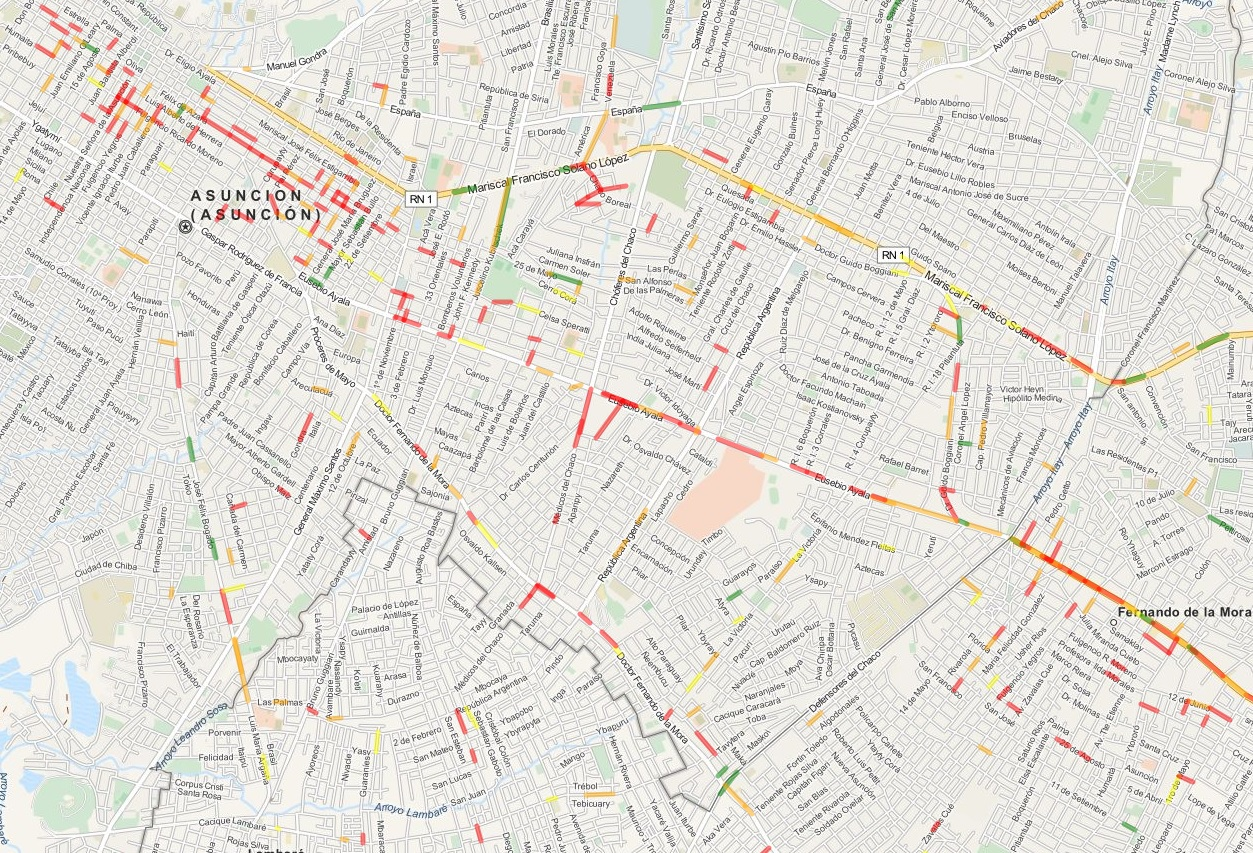
\includegraphics[width=0.7\textwidth]{capitulos/6/figuras/figura3.jpg}
	\caption{\label{fig:calles} Estado de calles en Autotracks}	
\end{figure}
